\documentclass{standalone}
\begin{document}

\section{Marco Teórico}

\subsection{Motores de videojuego}

\paragraph{}
Un motor de videojuego es un término que hace referencia a una serie de rutinas de programación, frameworks u otras herramientas, que permiten el diseño, la creación y la representación de un videojuego. La funcionalidad básica de un motor es proveer al videojuego de un motor de renderizado para los gráficos 2D y 3D, motor físico o detector de colisiones, sonidos, scripting, animación, inteligencia artificial, redes, streaming, administración de memoria y un escenario gráfico. El proceso de desarrollo de juegos es a menudo economizado, en gran parte, mediante la reutilización/adaptación del mismo motor de juego para crear diferentes juegos, o para facilitar la portabilidad de juegos a múltiples plataformas \cite{JasonGregory-GameEngineArchitecture}.

\paragraph{}
Algunos de los motores de juego mas usados en la actualidad, como lo son Source, Unity, Unreal Engine, GameMaker: Studio, CryEngine, entre otros, son conocidos por ser imperativos, siendo sus funciones mas importantes implementadas en lenguaje c++, lenguaje moderno conocido por ayudar en la ejecución de grandes proyectos.

\subsection{Programación Funcional}

\paragraph{}
Es un paradigma de programación, un estilo de construcción de la estructura y elementos de programas informáticos, que trata el cálculo como la evaluación de funciones matemáticas y evita el cambio de estado y datos mutables. Es un paradigma de programación declarativa, lo que significa que la programación se hace con expresiones o declaraciones. En código funcional, el valor de salida de una función sólo depende de los argumentos que se pasan a la función, por lo que llamar a una función f dos veces con el mismo valor para un argumento x producirá el mismo resultado f (x) cada vez. La eliminación de efectos secundarios, es decir, cambios en el estado que no dependen de las entradas de función, puede hacer mucho más fácil comprender y predecir el comportamiento de un programa, que es una de las motivaciones clave para el desarrollo de la programación funcional.

\paragraph{}
La programación funcional tiene su origen en el cálculo lambda, un sistema formal desarrollado en la década de 1930 para investigar la computabilidad, el problema de Entscheidung, la definición de funciones, la aplicación de funciones y la recursión. Muchos lenguajes de programación funcional pueden ser vistos como elaboraciones sobre el cálculo lambda.

%chequear nombre: funciones de primer orden
\subsubsection{Funciones de primera clase y de orden superior}
\paragraph{}
Funciones de orden superior son funciones que pueden tomar otras funciones como argumentos o devolverlos como resultados. Las funciones de orden superior están estrechamente relacionadas con las funciones de primera clase, en las cuales las funciones de orden superior y las funciones de primera clase pueden recibir como argumentos y generar como resultados otras funciones. Las funciones de orden superior describen un concepto matemático de funciones que operan sobre otras funciones, mientras que las funciones de primera clase son un término informático que describe las entidades del lenguaje de programación que no tienen ninguna restricción de su utilización.

\paragraph{}
Las funciones de orden superior permiten la aplicación parcial, una técnica en la que se aplica una función a sus argumentos uno a la vez, con cada aplicación devolver una nueva función que acepta el siguiente argumento. Esto le permite a uno expresar, por ejemplo, la función sucesor como el operador de suma aplicada parcialmente al número natural uno.

\subsubsection{Funciones puras}
\paragraph{}
También denominadas expresiones, son funciones que no tienen ningún efecto secundario, como alterar memoria o realizar operaciones de entrada o salida (E/S). Esto significa que las funciones puras tienen varias propiedades útiles, muchas de las cuales pueden ser utilizadas para optimizar el código:

\begin{itemize}
\item Si no se utiliza el resultado de una expresión pura, se puede eliminar sin afectar a otras expresiones.
\item El resultado es constante con respecto a la lista de parámetros, es decir, si la función pura se llama de nuevo con los mismos parámetros, el mismo resultado será devuelto, esto puede habilitar las optimizaciones de almacenamiento en caché.
\item Si no hay una dependencia de datos entre dos expresiones puras, entonces su orden puede ser invertido, o pueden llevarse a cabo en paralelo.
\end{itemize}

%evaluacion no estricta
\subsubsection{Evaluación perezosa}
\paragraph{}
Los argumentos a una función no se evalúan a menos que se utilicen realmente en la evaluación del cuerpo de la función. Ello ofrece un gran potencial para optimizaciones de parte de los compiladores y la posibilidad de evitar realizar ciertas operaciones.

\paragraph{}
Los lenguajes de evaluación tardía permiten la definición de estructuras de datos infinitas, algo que es mucho más complicado en un lenguaje de evaluación estricta. Por ejemplo, considera una lista con los números de Fibonacci. Está claro que no podemos realizar cálculos sobre una lista infinita en un tiempo razonable, o guardarla en memoria. Como el lenguaje es de evaluación tardía, solo las partes necesarias de la lista que son usadas realmente por el programa serán evaluadas. Esto permite abstraer muchos problemas y verlos desde una persepectiva de más alto nivel.

\subsubsection{Sistemas de tipos}
\paragraph{}
El uso de tipos de datos algebraicos y la coincidencia de patrones hace que la manipulación de estructuras de datos complejas convenientes y expresivos, la presencia de comprobaciones estrictas de tipos en tiempo de compilación hace que los programas sean más fiables, mientras que la inferencia de tipos libera al programador de la necesidad de declarar manualmente los tipos para el compilador al momento de declarar funciones u otras expresiones.

\subsection{Programación Funcional Reactiva}

\paragraph{}
La programación reactiva funcional (FRP, por sus siglas en ingles) es un enfoque elegante para especificar de forma declarativa los sistemas reactivos, que son sistemas orientados en la propagación de cambios de multiples entidades.

\paragraph{}
FRP integra la idea de flujo de tiempo y composición de eventos en la programación puramente funcional. Al manejar el flujo de tiempo de manera uniforme y generalizada, una aplicación obtiene claridad y fiabilidad. Así como la evaluación perezosa puede eliminar la necesidad de estructuras de control complejas, una noción uniforme de flujo de tiempo soporta un estilo de programación más declarativo que oculta un complejo mecanismo subyacente. Esto proporciona una manera elegante de expresar la computación en dominios como animaciones interactivas \cite{eh97:fran}, robótica \cite{Pembeci:2002:FRR:571157.571174}, visión por computadora, interfaces de usuario \cite{czaplicki2012elm} y simulación.

\subsubsection{FRP componentes básicos}

\paragraph{}
Para este proyecto de investigación se hará énfasis en la implementacion de FRP de la librería Yampa \cite{Courtney2003b}, que hace una implementacion de Arrowized FRP (AFRP), que es una mejora al FRP clásico, para mas detalles de la evolución de FRP leer \cite{czaplicki2012elm} capitulo 2.1.

\paragraph{Señales.}
En FRP una señal puede representar cualquier valor mutable. Estas pueden ser transformadas y combinadas, que a diferencia de otras soluciones mas tradiciones, permite abstraer varios detalles menores, permitiendo al programador lograr un mismo resultado usando menos código. En Yampa una señal es una función que que va de tiempo a valor, dicho en otras palabras, es una función que dado un tiempo determinado regresa el valor adecuado para el objeto mutable en el momento indicado. Un ejemplo es la posición del ratón.

\begin{equation}
Signal \ \alpha \approx Time \rightarrow \alpha
\end{equation}

\paragraph{Funciones de señal.}
Es una función que recibe una señal y produce otra señal. Estas funciones permiten alterar o generar nuevas señales dependiendo del estado actual de la señal original, por ejemplo, puede ser deseable generar una señal nueva cuando el ratón pasa por sobre algún elemento gráfico en especifico.

\begin{equation}
SF \ \alpha \ \beta \approx Signal \ \alpha \rightarrow Signal \ \beta
\end{equation}

\paragraph{Combinadores de funciones de señal.}
Similar a la composición de funciones, las SF pueden ser compuestas para permitir un mejor filtrado de las señales. En Yampa los combinadores mas comunes son:

\begin{itemize}
\item arr: crea un SF a partir de una función.
\item first: aplica una SF solo al primer elemento de la entrada y deja el resto sin cambios.
\item composición: compone dos SF, la señal resultada de la primera SF es dada como entrada a la segunda SF.
\item loop: crea una SF con memoria (Stateful) que interactua con su salida previa en cada ciclo.
\end{itemize}
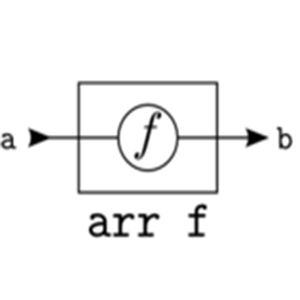
\includegraphics{Yampa-arr}
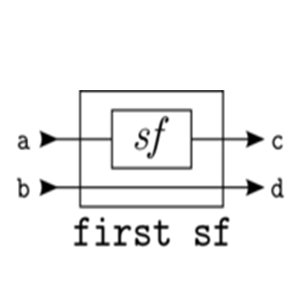
\includegraphics{Yampa-first}
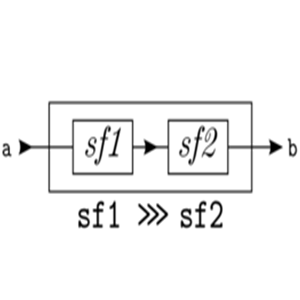
\includegraphics{Yampa-composition}
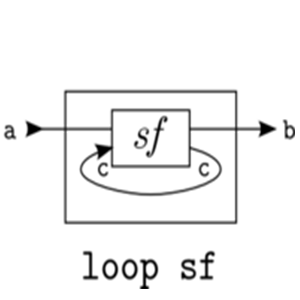
\includegraphics{Yampa-loop}
\paragraph{Suiches}
En una red de señales, es necesario poder cambiar su estructura conforme pasa el tiempo o se lleva a cabo ciertos eventos, los suiches permiten reflejar estos cambios aislando o activando ciertos elementos de la red.

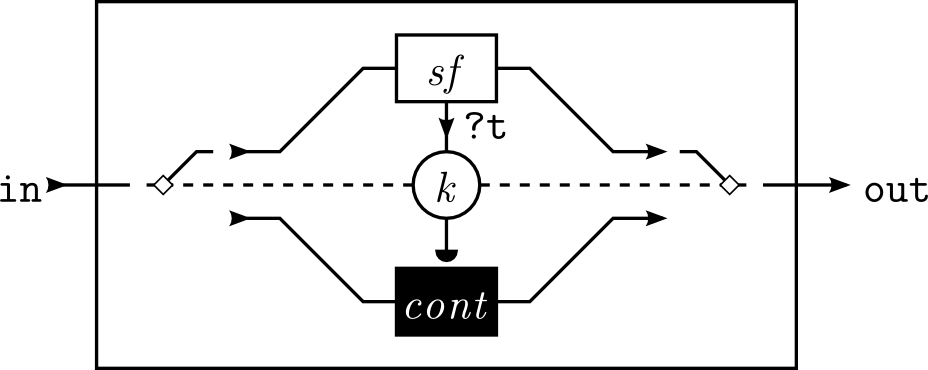
\includegraphics{Yampa-switch}

\end{document}
